\documentclass[12pt]{article}
\def\activityid{F05-X-v2}\usepackage[letterpaper,margin=.65in,top=.60in,bottom=.65in]{geometry}
\usepackage[T1]{fontenc}\usepackage[default]{sourcesanspro}
\usepackage{microtype,tikz,array,tabularx,fancyhdr,amsmath}\usepackage[hidelinks]{hyperref}
\usetikzlibrary{arrows.meta,calc}
\setlength{\parindent}{0pt}\setlength{\parskip}{7pt}\setlength{\headheight}{0pt}\setlength{\footskip}{26pt}\setlength{\emergencystretch}{2em}
\pagestyle{fancy}\fancyhf{}\renewcommand{\headrulewidth}{0pt}\renewcommand{\footrulewidth}{.4pt}
\fancyfoot[L]{\scriptsize Bellingham Math Circle / Week 5 / \activityid}\fancyfoot[R]{\scriptsize \thepage}
\definecolor{ink}{gray}{.12}\definecolor{soft}{gray}{.95}\color{ink}
\newcommand{\PageTitle}[2]{{\fontsize{10}{12}\selectfont\bfseries WEEK 5\quad TOWER LAB\hfill #1\par}\vspace{3pt}{\fontsize{26}{29}\selectfont\bfseries #2\par}\vspace{2pt}}
\newcommand{\NameLine}{{\small Name: \rule{2.65in}{.4pt}\hfill Date: \rule{1.35in}{.4pt}\par}\vspace{4pt}}
\newcommand{\Task}[2]{\par\vspace{3pt}{\large\bfseries #1}\par #2\par}
\newcommand{\Subhead}[1]{\par\vspace{3pt}{\large\bfseries #1}\par}
\newcommand{\RuleBox}[1]{\par\begingroup\setlength{\fboxsep}{8pt}\colorbox{soft}{\parbox{\dimexpr\linewidth-16pt\relax}{#1}}\endgroup\par}
\newcommand{\WriteBox}[2]{\par\textbf{#1}\par\vspace{2pt}\begin{tikzpicture}\draw[black!40,line width=.5pt] (0,0) rectangle (\dimexpr\linewidth-.5pt\relax,#2);\end{tikzpicture}\par}
\newcommand{\StudentFooter}{\vfill{\small Build first. Explain by pointing, talking, or drawing.}\par}
\newcommand{\Code}[1]{\texttt{#1}}

\hypersetup{pdftitle={Week 5: extra-grades-6-7}}
\begin{document}
\PageTitle{EXTRA / GRADES 6--7}{Small swaps force a lower bound}\NameLine
\RuleBox{New clue type: an entry clue fixes the height \textbf{in one cell}. There are no outside visibility clues. Rows and columns still contain 1--4 exactly once.}
\Task{1. A switch that preserves every rule.}{Copy this Latin square. In the upper-left 2-by-2 block, exchange the 1s and 2s. Why is the new square still legal?}\begin{center}\begin{minipage}{.47\linewidth}\centering 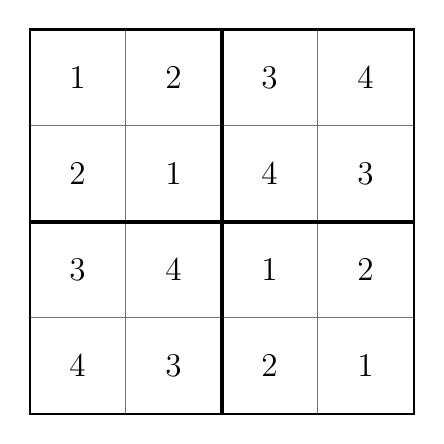
\begin{tikzpicture}[x=0.48in,y=0.48in]\draw[step=1,black!55] (0,0) grid (4,4);\draw[thick](0,0)rectangle(4,4);\draw[line width=1.4pt](2,0)--(2,4)(0,2)--(4,2);\node[font=\large]at(0.5,3.5){1};\node[font=\large]at(1.5,3.5){2};\node[font=\large]at(2.5,3.5){3};\node[font=\large]at(3.5,3.5){4};\node[font=\large]at(0.5,2.5){2};\node[font=\large]at(1.5,2.5){1};\node[font=\large]at(2.5,2.5){4};\node[font=\large]at(3.5,2.5){3};\node[font=\large]at(0.5,1.5){3};\node[font=\large]at(1.5,1.5){4};\node[font=\large]at(2.5,1.5){1};\node[font=\large]at(3.5,1.5){2};\node[font=\large]at(0.5,0.5){4};\node[font=\large]at(1.5,0.5){3};\node[font=\large]at(2.5,0.5){2};\node[font=\large]at(3.5,0.5){1};\end{tikzpicture}\end{minipage}\hfill\begin{minipage}{.47\linewidth}\centering 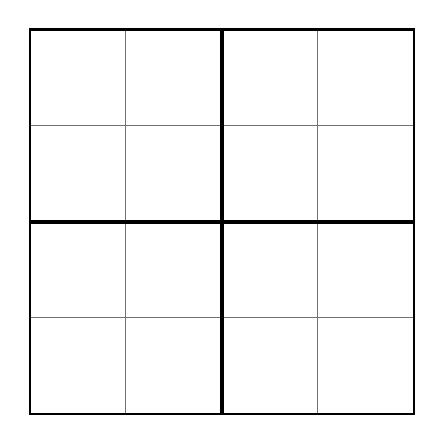
\begin{tikzpicture}[x=0.48in,y=0.48in]\draw[step=1,black!55] (0,0) grid (4,4);\draw[thick](0,0)rectangle(4,4);\draw[line width=1.4pt](2,0)--(2,4)(0,2)--(4,2);\end{tikzpicture}\end{minipage}\end{center}
\Task{2. Four independent hiding places.}{Each bold 2-by-2 block has a similar switch. Suppose you reveal at most three entry clues from the original square. Show that a second completion always remains.}
\WriteBox{Why must one whole switch escape the clues?}{.75in}
\Task{3. Is touching every block sufficient?}{Reveal just cells (row 1, column 1), (1,3), (3,1), (3,3). They touch all four bold blocks. Can you still make another square?}
\WriteBox{An alternative completion or a convincing reason:}{.75in}
\textbf{Go further:} A \emph{Latin trade} changes some entries and preserves every row and column. Explain why a uniquely determining entry set must touch every possible trade, not merely these four.\StudentFooter
\end{document}
